%-----------------------------------------------------------------
%	BASIC DOCUMENT LAYOUT
%-----------------------------------------------------------------
\documentclass[paper=a4, fontsize=12pt, twoside=semi, abstracton, listof=totoc, toc=left]{scrartcl}
\usepackage[T1]{fontenc}
\usepackage[utf8]{inputenc}
\usepackage{lmodern}
\usepackage{slantsc}
\usepackage{microtype}
\usepackage[british]{babel}
% \usepackage[backend=bibtex, style=phys, sorting=none, citestyle=authoryear, maxbibnames=3, maxcitenames=2]{biblatex}
\usepackage[backend=bibtex, style=trad-abbrv, sorting=none, maxbibnames=3, maxcitenames=2]{biblatex}
\addbibresource{bibliography.bib}
\makeatletter
	\def\blx@maxline{77}
\makeatother

% Sectioning layout
\addtokomafont{sectioning}{\normalfont\scshape}
\usepackage{tocstyle}
\usetocstyle{standard}
\renewcommand*\descriptionlabel[1]{\hspace\labelsep\normalfont\bfseries{#1}}
\usepackage[titletoc]{appendix}

% Empty pages
\usepackage{etoolbox}
% \pretocmd{\toc}{\cleardoubleevenemptypage}{}{}
% \pretocmd{\section}{\cleardoubleevenemptypage}{}{}
\pretocmd{\part}{\cleardoubleevenemptypage\thispagestyle{empty}}{}{}
\renewcommand\partheadstartvskip{\clearpage\null\vfil}
\renewcommand\partheadmidvskip{\par\nobreak\vskip 20pt\thispagestyle{empty}}

% Paragraph indentation behaviour
\setlength{\parindent}{0pt}
\setlength{\parskip}{0.3\baselineskip plus2pt minus2pt}
\newcommand{\sk}{\medskip\noindent}

% Fancy header and footer
\usepackage{fancyhdr}
\pagestyle{fancyplain}
\fancyhead[LO]{\thepage}
\fancyhead[CO]{}
\fancyhead[RO]{\nouppercase{\mytitle}}
\fancyhead[LE]{\nouppercase{\rightmark}}
% \fancyhead[LE]{\nouppercase{\leftmark}}
\fancyhead[CE]{}
\fancyhead[RE]{\thepage}
\fancyfoot{}
\renewcommand{\headrulewidth}{0.3pt}
\renewcommand{\footrulewidth}{0pt}
\setlength{\headheight}{13.6pt}

%-----------------------------------------------------------------
%	MATHS AND SCIENCE
%-----------------------------------------------------------------
\usepackage{amsmath,amsfonts,amsthm,amssymb}
\usepackage{xfrac}
\usepackage[a]{esvect}
\usepackage{chemformula}
\usepackage{graphicx}

\usepackage[arrowdel]{physics}
	\renewcommand{\vnabla}{\vec{\nabla}}
	% \renewcommand{\vectorbold}[1]{\boldsymbol{#1}}
	% \renewcommand{\vectorarrow}[1]{\vec{\boldsymbol{#1}}}
	% \renewcommand{\vectorunit}[1]{\hat{\boldsymbol{#1}}}
	\renewcommand{\vectorarrow}[1]{\vec{#1}}
	\renewcommand{\vectorunit}[1]{\hat{#1}}
	\renewcommand*{\grad}[1]{\vnabla #1}
	\renewcommand*{\div}[1]{\vnabla \vdot \va{#1}}
	\renewcommand*{\curl}[1]{\vnabla \cp \va{#1}}
	\let\rot\curl

% SI units
\usepackage[separate-uncertainty=true]{siunitx}
% \sisetup{range-phrase = \text{--}, range-units = brackets}
\sisetup{range-phrase = \text{--}, range-units = single}
\DeclareSIPrePower\quartic{4}
	%\DeclareSIUnit\micron{\micro\metre}

% Smaller trig functions
\newcommand{\Sin}{\trigbraces{\operatorname{s}}}
\newcommand{\Cos}{\trigbraces{\operatorname{c}}}
\newcommand{\Tan}{\trigbraces{\operatorname{t}}}

% Operator-style notation for matrices
\newcommand*{\mat}[1]{\hat{#1}}

% Matrices in (A|B) form via [c|c] option
\makeatletter
\renewcommand*\env@matrix[1][*\c@MaxMatrixCols c]{%
  \hskip -\arraycolsep
  \let\@ifnextchar\new@ifnextchar
  \array{#1}}
\makeatother

% Shorter \mathcal and \mathbb
\newcommand*{\mc}[1]{\mathcal{#1}}
\newcommand*{\mbb}[1]{\mathbb{#1}}

% Shorter ^\ast and ^\dagger
\newcommand*{\sast}{^{\star}{}}
\newcommand*{\sdag}{^{\dagger}{}}

% Blackboard bold identity
\usepackage{bbm}
\newcommand*{\bbid}{\mathbbm{1}}

% Shorter displaystyle
\newcommand*{\dsp}{\displaystyle}

% Inexact differential
\newcommand{\dbar}{\mathchar'26\mkern-12mu\mathrm{d}}
\newcommand{\indd}[1]{\dbar{#1}}

% Arrows with text and cancels for developments
\newcommand{\tikzmark}[1]{\tikz[overlay,remember picture] \node (#1) {};}
\tikzset{square arrow/.style={to path={-- ++(0,-.25) -| (\tikztotarget)}}}
\usepackage{cancel}

\newcommand*\acr[1]{\textscale{.85}{#1}}

%-----------------------------------------------------------------
%	OTHER PACKAGES
%-----------------------------------------------------------------
\usepackage{environ}

%Left numbered equations
\makeatletter
	\NewEnviron{Lalign}{\tagsleft@true\begin{align}\BODY\end{align}}
\makeatother

% Plots and graphics
\usepackage{pgfplots}
\usepackage{tikz}
\usepackage{color}
	\makeatletter
		\color{black}
		\let\default@color\current@color
	\makeatother

% Richer enumerate, figure, and table support
\usepackage{enumerate}
\usepackage[shortlabels]{enumitem}
\usepackage{float}
\usepackage{tabularx}
\usepackage{booktabs}
	%\setlength{\intextsep}{8pt}
% \numberwithin{equation}{section}
% \numberwithin{figure}{section}
% \numberwithin{table}{section}

% No indentation after certain environments
\makeatletter
\newcommand*\NoIndentAfterEnv[1]{%
	\AfterEndEnvironment{#1}{\par\@afterindentfalse\@afterheading}}
\makeatother
%\NoIndentAfterEnv{thm}
\NoIndentAfterEnv{defi}
\NoIndentAfterEnv{example}
\NoIndentAfterEnv{table}

% Misc packages
\usepackage{ccicons}
\usepackage{lipsum}
\usepackage{todonotes}
\usepackage{array}
\usepackage{multirow}

% Print DOI only if there's no URL
\renewbibmacro*{doi+eprint+url}{%
  \iftoggle{bbx:doi}
    {\iffieldundef{url}{\printfield{doi}}{}}
    {}%
  \newunit\newblock
  \iftoggle{bbx:eprint}
    {\usebibmacro{eprint}}
    {}%
  \newunit\newblock
  \iftoggle{bbx:url}
    {\usebibmacro{url+urldate}}
    {}}

%-----------------------------------------------------------------
%	SYNTAX HIGHLIGHTING
%-----------------------------------------------------------------
\usepackage[formats]{listings}
\usepackage{relsize}
\usepackage{chngcntr}

\renewcommand{\lstlistingname}{Snippet}
\renewcommand{\lstlistlistingname}{List of snippets}

\lstloadlanguages{C,bash}

\newcommand*{\inline}{\lstinline[basicstyle=\normalsize\ttfamily]}


\lstset{language=C,
		frame=tb,
		% captionpos=b,
		tabsize=2,
		% showtabs=true,
		breaklines=true,
		breakatwhitespace=true,
		basicstyle=\smaller\ttfamily,
		numbers=left,
		numberstyle=\tiny,
		numbersep=7.5pt,
		% commentstyle=\textsl,
		xleftmargin=3ex}
\lstset{escapeinside={(*}{*)}}   % for (*\ref{ }*) inside lstlistings (Scode)

\lstdefinestyle{output}{
	language=,
	% showtabs=true,
	% showspaces=true,
	numbers=none,
	frame=tblr,
	% columns=fullflexible,
	% backgroundcolor=\color{blue!10},
	numbers=none,
	xleftmargin=3ex}

\expandafter\patchcmd\csname \string\lstinline\endcsname{%
	\leavevmode
	\bgroup
}{%
	\leavevmode
	\ifmmode\hbox\fi
	\bgroup
}{}{%
	\typeout{Patching of \string\lstinline\space failed!}%
}
%% end of patch

%-----------------------------------------------------------------
%	THEOREMS
%-----------------------------------------------------------------
\usepackage{thmtools}

% Theroems layout
\declaretheoremstyle[
	spaceabove=6pt, spacebelow=6pt,
	headfont=\normalfont,
	notefont=\mdseries, notebraces={(}{)},
	bodyfont=\small,
	postheadspace=1em,
]{small}

\declaretheorem[style=plain,name=Theorem,qed=$\square$,numberwithin=section]{thm}
\declaretheorem[style=plain,name=Corollary,qed=$\square$,sibling=thm]{cor}
\declaretheorem[style=plain,name=Lemma,qed=$\square$,sibling=thm]{lem}
\declaretheorem[style=definition,name=Definition,qed=$\blacksquare$,numberwithin=section]{defi}
\declaretheorem[style=definition,name=Example,qed=$\blacktriangle$,numberwithin=section]{example}
\declaretheorem[style=small,name=Proof,numbered=no,qed=$\square$]{sproof}

%-----------------------------------------------------------------
%	ELA MOTHERFUCKING GEMINADA
%-----------------------------------------------------------------
\def\xgem{%
	\ifmmode
		\csname normal@char\string"\endcsname l%
	\else
		\leftllkern=0pt\rightllkern=0pt\raiselldim=0pt
		\setbox0\hbox{l}\setbox1\hbox{l\/}\setbox2\hbox{.}%
		\advance\raiselldim by \the\fontdimen5\the\font
		\advance\raiselldim by -\ht2
		\leftllkern=-.25\wd0%
		\advance\leftllkern by \wd1
		\advance\leftllkern by -\wd0
		\rightllkern=-.25\wd0%
		\advance\rightllkern by -\wd1
		\advance\rightllkern by \wd0
		\allowhyphens\discretionary{-}{}%
		{\kern\leftllkern\raise\raiselldim\hbox{.}%
			\kern\rightllkern}\allowhyphens
	\fi
}
\def\Xgem{%
	\ifmmode
		\csname normal@char\string"\endcsname L%
	\else
		\leftllkern=0pt\rightllkern=0pt\raiselldim=0pt
		\setbox0\hbox{L}\setbox1\hbox{L\/}\setbox2\hbox{.}%
		\advance\raiselldim by .5\ht0
		\advance\raiselldim by -.5\ht2
		\leftllkern=-.125\wd0%
		\advance\leftllkern by \wd1
		\advance\leftllkern by -\wd0
		\rightllkern=-\wd0%
		\divide\rightllkern by 6
		\advance\rightllkern by -\wd1
		\advance\rightllkern by \wd0
		\allowhyphens\discretionary{-}{}%
		{\kern\leftllkern\raise\raiselldim\hbox{.}%
			\kern\rightllkern}\allowhyphens
	\fi
}

\expandafter\let\expandafter\saveperiodcentered
	\csname T1\string\textperiodcentered \endcsname

\DeclareTextCommand{\textperiodcentered}{T1}[1]{%
	\ifnum\spacefactor=998
		\Xgem
	\else
		\xgem
	\fi#1}

%-----------------------------------------------------------------
%	DEDICATION ENVIRONMENT
%-----------------------------------------------------------------

\newenvironment{mydedication}
	{\clearpage           % we want a new page
	\thispagestyle{empty}% no header and footer
	\vspace*{\stretch{1}}% some space at the top
	\itshape             % the text is in italics
	\raggedleft          % flush to the right margin
	}
	{\par % end the paragraph
	\vspace{\stretch{3}} % space at bottom is three times that at the top
	\clearpage           % finish off the page
	}

%-----------------------------------------------------------------
%	PDF INFO AND HYPERREF
%-----------------------------------------------------------------
\usepackage{hyperref}
\hypersetup{colorlinks, citecolor=black, filecolor=black, linkcolor=black, urlcolor=black}
\usepackage{cleveref}
	\crefname{section}{\S}{\SS}
	\Crefname{section}{\S}{\SS}
	\crefname{listing}{snippet}{}

\newcommand*{\mytitle}{Parallel Programming: GPU}
\newcommand*{\mysubtitle}{Assignment 4}
\newcommand*{\myauthor}{Alfredo Hernández \and Alejandro Jiménez}
% \newcommand*{\mysupervisor}{J. Minguillón}
% \newcommand*{\mytutor}{}
\newcommand*{\myuni}{Universitat Autònoma de Barcelona}
\newcommand*{\mydate}{28th January}

\pdfstringdefDisableCommands{\def\and{and }}

\usepackage{hyperxmp}
\hypersetup{pdfauthor={\myauthor}, pdftitle={\mytitle: \mysubtitle}}

%-----------------------------------------------------------------
%	TITLE SECTION AND DOCUMENT BEGINNING
%-----------------------------------------------------------------
\newcommand{\horrule}[1]{\rule{\linewidth}{#1}}
\title{
	\normalfont
	\small \scshape{\myuni} \\ [25pt]
	\horrule{0.5pt} \\ [0.4cm]
	\huge \mytitle \\
	\Large \scshape{\mysubtitle} \\
	\horrule{2pt} \\ [0.5cm]
}
\author{\myauthor }
% \\ \footnotesize Supervised by: \mysupervisor \\ \footnotesize Academic tutor: \mytutor}
\date{\mydate}

\begin{document}

%\counterwithin{lstlisting}{section}

\clearpage\maketitle
\thispagestyle{empty}
\addtocounter{page}{-1}

%-----------------------------------------------------------------
%	DEDICATION
%-----------------------------------------------------------------
% \begin{mydedication}
% 	Dedicated to RMT, Val \& the Brotherhood
% \end{mydedication}

%-----------------------------------------------------------------
%	DOCUMENT BODY
%-----------------------------------------------------------------
% \cleardoubleevenemptypage
\include{./contents/0-abstract}

\pdfbookmark[1]{\contentsname}{toc}
\tableofcontents

%-----------------------------------------------------------------
%	INTRODUCTION
%	!TEX root = ./../main.tex
%-----------------------------------------------------------------
\section{Introduction}

In this assignment we aim to improve the execution time of the now-common Laplace 2D code and measure the impact of using MPI.

In order to make the biggest difference on the code and fully appreciate the power of parallel computing, we chose the most computational demanding loop and created many threads using OpenMP, which would split the iterations into different, parallel, more efficient processes. Nextly, we would add MPI orders in as many loops as we did found useful. 

Eventually, We will measure the impact of the parallelisation of the code using and more sophisticated analytical tools such as \emph{TAU}. Using \emph{TAU} we will try to identify and analyse the different internal operations of the code and how their performance varies when using a different number of threads.


% Moreover, we tested different numbers of threads and many scheduling methods.

% Finally, we recorded the execution times for every alteration in the paralleling in order to be able to compare different paralleling metodologies and decide which method performed the better on our code.



%-----------------------------------------------------------------
%	PERFORMANCE
%	!TEX root = ./../main.tex
%-----------------------------------------------------------------
\section{Implementation of MPI}

\subsection{Setting up the system before working}

Before doing anything, we need to load the \inline{modules} of the compiler and libraries we have to use:
\begin{lstlisting}[language=bash]
module load gcc/6.1.0
module load openmpi/1.8.1
\end{lstlisting}

We need to compile the \inline{Makefile} to use TAU with MPI:
\begin{lstlisting}[language=bash]
cd tau-2.26
./configure -prefix=/home/master/ppM/ppM-1-10/my_TAU -mpi
export PATH=/home/master/ppM/ppM-1-10/my_TAU/x86_64/bin:$PATH
make install
\end{lstlisting}

We need to export the Makefile to the environment variable to be able to use TAU with MPI whilst compiling and running our C program, as well as the \inline{optCompInst} option:
\begin{lstlisting}[language=bash]
export TAU_MAKEFILE=/home/master/ppM/ppM-1-10/my_TAU/x86_64/lib/ Makefile.tau-mpi
export TAU_OPTIONS=-optCompInst
\end{lstlisting}

%-----------------------------------------------------------------
\subsection{Parallelisation with MPI}

To compile an MPI program we would usually compile the C code using \inline{mpicc}:
\begin{lstlisting}[language=bash]
mpicc -lm laplaceMPI.c -o compiledfile
\end{lstlisting}

However, to use TAU, we need to compile it using
\begin{lstlisting}[language=bash]
tau_cc.sh -lm laplaceMPI.c -o compiledfile
\end{lstlisting}

One of the main variables to consider when improving the performance of a code using MPI is the number of threads that we use. Specifying the exact number of threads to be used can be done easily when running the compiled  file. 

In the following snippet it is showed how to run the compiled code over a $1000 \times 1000$ matrix using $4$ threads.

\begin{lstlisting}[language=bash]
mpirun -np 4 compiledfile 1000
\end{lstlisting}

An important difference between the usage of OpenMP and MPI is that we specify the number of threads within the very code in the former, whereas we set the number of threads when executing the compiled file in the latter.

Using MPI we can improve greatly the performance of the code when used on sequential portions of the program, such as loops where each step is independent from the others.

\bigskip

In the proceeding section, we will explain our implementation of MPI to parallelise the code to solve 2D Laplace equation using Jacobi Iteration method.

%-----------------------------------------------------------------
\subsection{Basic parallel solution}

Suppose that we are going to use $N$ processes to solve the problem in a distributed way. Accordingly with the characteristics of the problem, each of these processes will have to carry on the computation over a portion of the matrix $A$, taking care for interchanging the necessary data and synchronising with other processes. The specific processes that will have to communicate will depend on how the data is partitioned among them.

The simplest partition of $A$ is shown in figure \ref{fig:a-matrix}. In this case, each process $P_{i}$ takes care of the computation of $m/N$ rows of $A$ and, in the general case ($0 < i < N-1$), it needs the last row of $P_{i-1}$ and the first of $P_{i+1}$.

\begin{figure}[H]
    \centering
    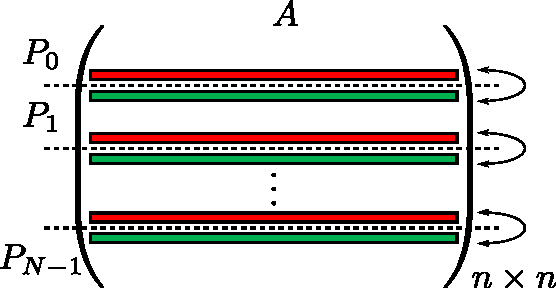
\includegraphics[width=0.45\textwidth]{images/a-matrix}
    \caption{Diagram of the partition of the matrix $A$}
    \label{fig:a-matrix}
\end{figure}

First of all, we need to define some variables in our C program that are needed for the MPI implementation, like \inline{rank}, \inline{size}, \inline{m}, \inline{ri}, \inline{rf}; and to initialize the MPI parallel region:

\begin{lstlisting}[firstnumber=52]
 // Variables needed for MPI
int rank, size;
\end{lstlisting}

We define the initial and final row of the subpartitions of the matrix as
\begin{align}
\begin{aligned}
    r_{i}[k] &= \frac{n}{N} \times \qty k \\
    r_{f}[k] &= \qty( \frac{n}{N} \times (k + 1) ) - 1 \\
\end{aligned}        
\end{align}
where $n$ is the dimension of the matrix, $N$ (or \inline{size}) is the amount of threads used, and $k = 0, \dots, N-1$ (or \inline{rank}) is the number of the working thread. Notice that Thread 0 will be used to make calculations as well as being the master thread to coordinate all computations. Notice that $n/N$ must be an integer.
 
\begin{lstlisting}[firstnumber=75]
// Initialisation of MPI parallel region
MPI_Init(&argc, &argv);
MPI_Comm_rank(MPI_COMM_WORLD, &rank);
MPI_Comm_size(MPI_COMM_WORLD, &size);
MPI_Status status;

// Define the partition of the matrix
int m = n/size;
int ri = rank * m, 
int rf = (rank+1) * m-1;
\end{lstlisting}

In the main loop of the program, we implement the basic parallel solution as described above. In the snippets below we can see excerpts of the script where MPI has been used. The rest of the program is almost identical to the standard implementation without MPI.

We can send and recieve messages from the different threads:
\begin{lstlisting}[firstnumber=96]
// Interchange of messages between consecutive rows
if ( rank > 0 ) {
	MPI_Send(&A[ri*n], n, MPI_FLOAT, rank-1, 1, MPI_COMM_WORLD);
	MPI_Recv(&A[(ri-1)*n], n, MPI_FLOAT, rank-1, 2, MPI_COMM_WORLD, &status);
}
if ( rank < size-1 ) {
	MPI_Send(&A[rf*n], n, MPI_FLOAT, rank+1, 2, MPI_COMM_WORLD);
	MPI_Recv(&A[(rf+1)*n], n, MPI_FLOAT, rank+1, 1, MPI_COMM_WORLD, &status);
}
\end{lstlisting}

The main part of the program, performing the Laplace step function using the implemented partition of the matrix $A$:
\begin{lstlisting}[firstnumber=106]
// Computation of the Laplace Step using MPI
if ( rank == 0 ) {
	for ( j = ri+1; j <= rf; j++ ) {
		for ( i = 1; i < n-1; i++ ) {
			temp[j*n+i] = stencil(A[j*n+i+1], A[j*n+i-1], A[(j-1)*n+i], A[(j+1)*n+i]);
			error = max_error( error, temp[j*n+i], A[j*n+i] );
		}
	}
}
if ( rank == (size-1) ) {
	for ( j = ri; j < rf; j++ ) {
		for ( i=1; i < n-1; i++ ) {
			temp[j*n+i] = stencil(A[j*n+i+1], A[j*n+i-1], A[(j-1)*n+i], A[(j+1)*n+i]);
			error = max_error( error, temp[j*n+i], A[j*n+i] );
		}
	}
}
if ( rank != 0 && rank != (size-1) ) {
	for ( j = ri; j <= rf; j++ ) {
		for ( i = 1; i < n-1; i++ ) {
			temp[j*n+i] = stencil(A[j*n+i+1], A[j*n+i-1], A[(j-1)*n+i], A[(j+1)*n+i]);
			error = max_error( error, temp[j*n+i], A[j*n+i] );
		}
	}
}
\end{lstlisting}

We send the partial errors of each thread to the master:
\begin{lstlisting}[firstnumber=132]
// Sending partial errors to the master and computing the maximum to find the global error
if ( rank != 0 ) {
		MPI_Send(&error, 1, MPI_FLOAT, 0, 3, MPI_COMM_WORLD);
} else {
	errors[0] =error;
	for (i = 1; i < size; i++ ) {
		MPI_Recv(&errors[i], 1, MPI_FLOAT, i, 3, MPI_COMM_WORLD, &status);
	}
}
global_error = maximum(errors, size);
\end{lstlisting}

The master calcualtes the global error using the partial errors previously sent:
\begin{lstlisting}[firstnumber=143]
// Sending back the resulting error
if ( rank == 0 ) {
	for(i = 1; i<size; i++ ) MPI_Send(&global_error, 1, MPI_FLOAT, i, 4, MPI_COMM_WORLD);
} else {
	MPI_Recv(&global_error, 1, MPI_FLOAT, 0, 4, MPI_COMM_WORLD, &status);
}
\end{lstlisting}

As usual, once we've finished the computations, we need to \emph{close} MPI.
\begin{lstlisting}[firstnumber=156]
MPI_Finalize();
\end{lstlisting}

As it can be seen, it is almost the same algorithm implemented in the provided \inline{lapFusion.c} code, just distributing the work and adding the data interchange among processes.
%-----------------------------------------------------------------
%	PERFORMANCE
%	!TEX root = ./../main.tex
%-----------------------------------------------------------------
\section{Analysis of 2D Laplace program}\label{sec:results-laplace}

%-----------------------------------------------------------------
\subsection{CPU versions of the program}
To ease the work with the different versions of the code, we will use a systematic naming structure for the source codes, the binaries, and the logs:
\begin{itemize}
	\item \inline{lapCPU[#number]-description.c}
	\item \inline{lapCPU[#number]}
	\item \inline{lapCPU[#number]-perf.log}
\end{itemize}

This systematic naming convention will allow us to analyse the results easily using bash, AWK (using \inline{extract_perf.awk}), and R.

%---------------------------------
\subsubsection{Baseline \texttt{laplace2d.c} (\texttt{lapCPU1})}
First of all, we use the baseline \inline{laplace2d.c} program as provided by the professors:
\begin{lstlisting}[language=bash]
pgcc -lm -fast -Minfo=all lapCPU1-baseline.c -o lapCPU1
perf stat ./lapCPU1 250 2> lapCPU1-perf.log
\end{lstlisting}

The PGI compiler performs a series of optimisations on the code generated for CPU. The most relevant performance metrics are the elapsed execution time (\SI{135.33}{\s}), the total number of executed machine instructions (\num{40.26e9}), and the IPC rate (\num{0.09}).

%---------------------------------
\subsubsection{Baseline \texttt{lapFusion} (\texttt{lapCPU2} \& \texttt{lapCPU3})}
The second analysed version of the code is using the baseline \inline{lapFusion.c} program as provided by the professors:
\begin{lstlisting}[language=bash]
pgcc -lm -fast -openmp -Minfo=all lapCPU2-Fusion-baseline.c -o lapCPU2
perf stat ./lapCPU2 4096 250 2> lapCPU2-perf.log
\end{lstlisting}

The execution time is significantly reduced from \SI{135.33}{\s} to \SI{17.06}{\s}, but the total number of executed instructions is multiplied by 2.75 (\num{109.06e9}). This is something that we must check. A detailed look at the output from the PGI compiler reveals that the optimised code is not vectorized, even with the OpenMP \inline{#pragma} that confirms that the loop in line 23 is vectorisable.

In order to improve the task of the compiler, we include the \inline{inline} keyword before the declaration of functions \inline{stencil()} and \inline{max_error()} in the \inline{lapFusion.c} code, and it is compiled and executed again:
\begin{lstlisting}[language=bash]
pgcc -lm -fast -openmp -Minfo=all lapCPU3-Fusion-good.c -o lapCPU3
perf stat ./lapCPU3 4096 250 2> lapCPU3-perf.log
\end{lstlisting}

Again, the execution time is reduced from \SI{17.06}{\s} to \SI{9.43}{\s}, and the total number of executed instructions is almost halved (\num{56.66e9}), but still the optimised code is not vectorised. The compiler is not able to make a good analysis of the data dependencies when the matrices are represented as one-dimensional vectors and the elements are addressed using complex expressions.

Instead of trying to improve the output from the PGI compiler we opt by using the GCC compiler.

%---------------------------------
\subsubsection{Parallelised \texttt{lapFusion} using OpenMP (\texttt{lapCPU4})}
First of all, we need to load the GCC compiler into the system:
\begin{lstlisting}[language=bash]
module load gcc/7.2.0
\end{lstlisting}

Now, we create a parallelised version of the \inline{lapFusion} code using the following \inline{#pragma} directives:
\begin{lstlisting}[firstnumber=24]
  #pragma omp parallel for num_threads(3)
  for ( j=1; j < n-1; j++ )
	#pragma omp simd reduction(max:error)
	for ( i=1; i < n-1; i++ )
\end{lstlisting}

Then we compile using the GCC compiler and execute as usual:
\begin{lstlisting}[language=bash]
gcc -Ofast -lm -fopenmp lapCPU4-Fusion-parallel.c -o lapCPU4
perf stat ./lapCPU4 4096 250 2> lapCPU4-perf.log
\end{lstlisting}

Notice that using the \inline{inline} keyword has a very small influence on the execution time when vectorising the code using OpenMP.

The execution with three threads for 250 convergence loop iterations is about $2.2$ times faster than using a single thread and the operations have indeed been divided by 3 (\num{19.24e9}).

The fact that the performance does not scale linearly with the number of threads indicates that there is a performance problem. Since the total number of instructions executed is almost the same, the problem is an unexpected reduction of the IPC rate: some instructions are executed slower when using three processing cores than when using only one core. The explanation is that the DRAM memory bandwidth is almost exhausted with a single thread, and therefore the performance is bounded by the peak bandwidth of the DRAM memory.

%---------------------------------
\subsubsection{Comparison of the CPU versions}
In figure \ref{fig:times-cpu} below we can see a visual comparison of the execution times of the CPU versions of the Laplace program. The execution time is computed for \num{10000} iterations of the convergence loop, which is extrapolated by multiplying by 40 the time for executing 250 iterations of the convergence loop.
\begin{figure}[H]
	\centering
	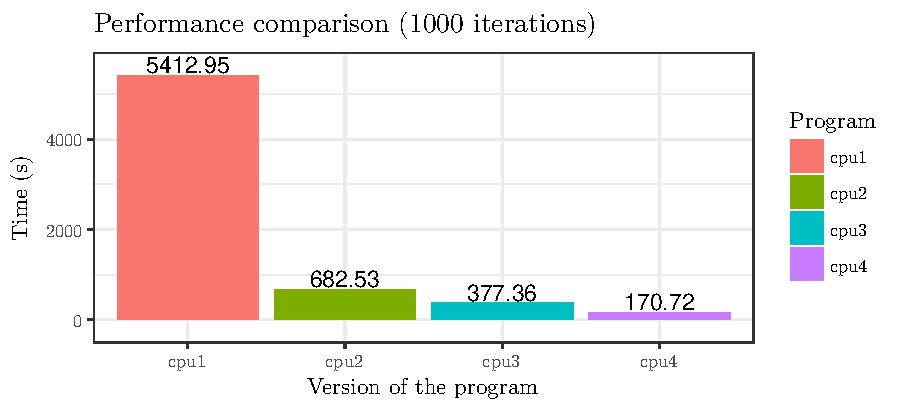
\includegraphics[width=0.9\textwidth]{images/times-cpu}
	\caption{Execution times of the CPU versions of the program}
	\label{fig:times-cpu}
\end{figure}

In the figure we can clearly see how each of the improvements has resulted in a reduction of the compilation time, specially the change from the sequential \inline{laplace2d.c} version to the \inline{lapFusion.c} version.

%-----------------------------------------------------------------
\subsection{GPU versions of the program}
To ease the work with the different versions of the code, we will use a systematic naming structure for the source codes, the binaries, and the compiler and profiler logs:
\begin{itemize}
	\item \inline{lapGPU[#number]-description.c}
	\item \inline{lapGPU[#number]}
	\item \inline{lapGPU[#number]-comp.log}
	\item \inline{lapGPU[#number]-nvp.log}
	\item \inline{lapGPU[#number]-metrics.log}
\end{itemize}

This systematic naming convention will allow us to analyse the results easily using bash, AWK (using \inline{extract_nvp.awk}), and R.

%---------------------------------
\subsubsection{Baseline (\texttt{lapGPU1})}
For this part, we will make our modifications using \inline{#pragma} directives on the \inline{laplace2d.c} code.

\begin{lstlisting}[firstnumber=77]
while ( error > tol && iter < iter_max )
{
	#pragma acc kernels
	for( i=1; i < m-1; i++ )
		for( j=1; j < n-1; j++)
			Anew[j][i] = ( A[j][i+1]+A[j][i-1]+A[j-1][i]+A[j+1][i]) / 4;

	error = 0.f;
	#pragma acc kernels
	for( i=1; i < m-1; i++ )
		for( j=1; j < n-1; j++)
			error = fmaxf( error, sqrtf( fabsf( Anew[j][i]-A[j][i] ) ) );

	#pragma acc kernels
	for( i=1; i < m-1; i++ )
		for( j=1; j < n-1; j++)
			A[j][i] = Anew[j][i];

	iter++;
	if(iter % (iter_max/10) == 0) printf("%5d, %0.6f\n", iter, error);
}
\end{lstlisting}

Since we will use the GPU for the calculations, we must use the PGI compiler:
\begin{lstlisting}[language=bash]
pgcc -fast -acc -ta=tesla:cc30 -Minfo=accel lapGPU1-baseline.c -o lapGPU1 &> lapGPU1-comp.log
\end{lstlisting}

Then we can use \inline{nvprof} to extract performance stats and some useful metrics:
\begin{lstlisting}[language=bash]
nvprof ./lapGPU1 10000 2> lapGPU1-nvp.log
nvprof --kernels "main_82_gpu" --metrics sm_activity,inst_executed,l2_utilization, dram_utilization,dram_read_throughput,dram_write_throughput,ipc ./lapGPU1 100 2> lapGPU1-metrics.log
\end{lstlisting}

The first thing to notice is that if we only use \inline{#pragma acc kernels} directives before each of the loops, most of the computation time is wasted on copying memory from the CPU to the GPU (and the other way around) for each iteration, as seen in figure~\ref{fig:timeline-gpu1b} below.
\begin{figure}[H]
	\centering
	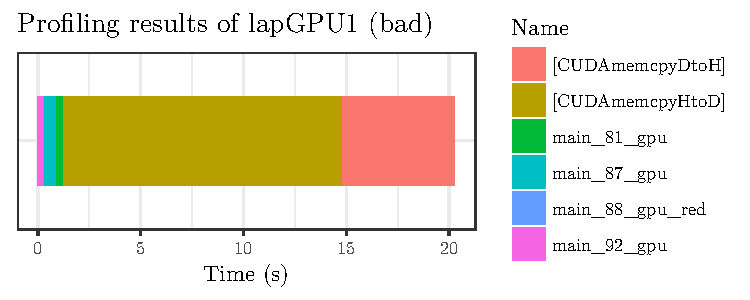
\includegraphics[width=0.7\textwidth]{images/timeline-gpu1b}
	\caption{Timeline of the execution time of the GPU1 version (bad), for 250 iterations}
	\label{fig:timeline-gpu1b}
\end{figure}

To fix this, we also need to include the following \inline{#pragma} directive before the main \inline{while} loop to tell the program that the GPU already has all the variables; this way the memory is only copied once from the CPU to the GPU at the beginning, and from the GPU to the CPU when the program finishes:
\begin{lstlisting}[firstnumber=77]
#pragma acc data copyin(A,Anew)
while ( error > tol && iter < iter_max )
\end{lstlisting}

In this way, we reduce the copying time to a bare minimum, as seen in figure~\ref{fig:timeline-gpu1} below. Even though we do 40 times the amount of iterations, the time is only doubled. This is a clear indication that we are using the GPU almost purely for calculations.
\begin{figure}[H]
	\centering
	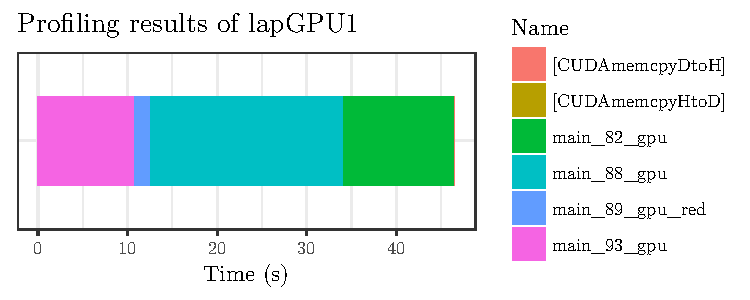
\includegraphics[width=0.7\textwidth]{images/timeline-gpu1}
	\caption{Timeline of the execution time of the GPU1 version, for \num{10000} iterations}
	\label{fig:timeline-gpu1}
\end{figure}

%---------------------------------
\subsubsection{Optimisation: loop fusion (\texttt{lapGPU2})}

For this version of the program, we fuse the loop for the calculation of the next step and the error into one single loop:
\begin{lstlisting}[firstnumber=81]
#pragma acc kernels
		for( i=1; i < m-1; i++ )
			for( j=1; j < n-1; j++){
				Anew[j][i] = ( A[j][i+1]+A[j][i-1]+A[j-1][i]+A[j+1][i]) / 4;
				error = fmaxf( error, sqrtf( fabsf( Anew[j][i]-A[j][i] ) ) );}
\end{lstlisting}

Then we compile with the PGI compiler as usual, and extract performance and metrics information:
\begin{lstlisting}[language=bash]
pgcc -fast -acc -ta=tesla:cc30 -Minfo=accel lapGPU2-loopfusion.c -o lapGPU2 &> lapGPU2-comp.log
nvprof ./lapGPU2 10000 2> lapGPU2-nvp.log
nvprof --kernels "main_82_gpu" --metrics sm_activity,inst_executed,l2_utilization, dram_utilization,dram_read_throughput,dram_write_throughput,ipc ./lapGPU2 100 2> lapGPU2-metrics.log
\end{lstlisting}

In figure~\ref{fig:timeline-gpu2} below we can clearly see how the two loops have been fused into one single operation, and how this fused operation is faster than the two operations by themselves in figure~\ref{fig:timeline-gpu1}. Notice that the reduction operation and the one done in \inline{main_93_gpu} have essentially the same duration in both implementations.
\begin{figure}[H]
	\centering
	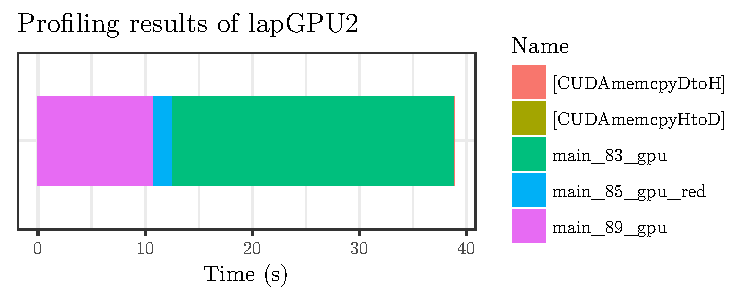
\includegraphics[width=0.7\textwidth]{images/timeline-gpu2}
	\caption{Timeline of the execution time of the GPU2 version, for \num{10000} iterations}
	\label{fig:timeline-gpu2}
\end{figure}

%---------------------------------
\subsubsection{Optimisation: loop interchange (\texttt{lapGPU3})}
For this version, we just exchange the order of the nested loops in lines \numrange{82}{83} and \numrange{88}{89}:
\begin{minipage}{.45\textwidth}
\begin{lstlisting}[firstnumber=81]
for( i=1; i < m-1; i++ )
	for( j=1; j < n-1; j++){
\end{lstlisting}
\end{minipage}%
\begin{minipage}{0.1\textwidth}
$\,\,\quad\mapsto$
\end{minipage}%
\begin{minipage}{0.45\textwidth}
\begin{lstlisting}[firstnumber=81]
for( j=1; j < n-1; j++ )
	for( i=1; i < m-1; i++){
\end{lstlisting}
\end{minipage}

Then we compile with the PGI compiler as usual, and extract performance and metrics information:
\begin{lstlisting}[language=bash]
pgcc -fast -acc -ta=tesla:cc30 -Minfo=accel lapGPU3-loopinter.c -o lapGPU3 &> lapGPU3-comp.log
nvprof ./lapGPU3 10000 2> lapGPU3-nvp.log
nvprof --kernels "main_83_gpu" --metrics sm_activity,inst_executed,l2_utilization, dram_utilization,dram_read_throughput,dram_write_throughput,ipc ./lapGPU3 100 2> lapGPU3-metrics.log
\end{lstlisting}

Having a look at figure~\ref{fig:timeline-gpu3} below and comparing it to figure~\ref{fig:timeline-gpu2}, we see no major improvements; one could even say that the performance is a bit worse.
\begin{figure}[H]
	\centering
	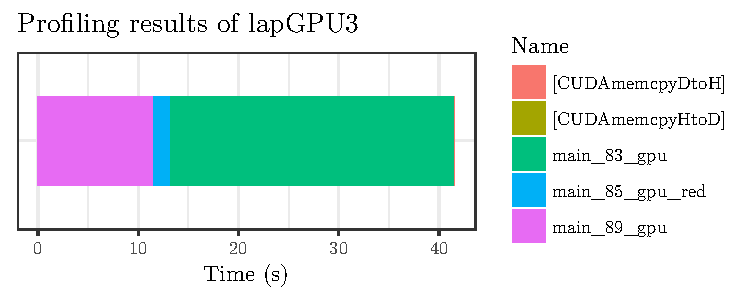
\includegraphics[width=0.7\textwidth]{images/timeline-gpu3}
	\caption{Timeline of the execution time of the GPU3 version, for \num{10000} iterations}
	\label{fig:timeline-gpu3}
\end{figure}

The reason for not being any major improvement is that the PGI compiler already knows the “good” order of the loops when it compiles the program.

%---------------------------------
\subsubsection{Optimisation: \texttt{sqrt} out of the loop (\texttt{lapGPU4})}
For this version, we move the $\sqrt{\texttt{error}}$ outside of the loop, since we do not need to know the square root of the intermediate errors, just the final error:
\begin{lstlisting}[firstnumber=82]
for( i=1; i < m-1; i++ )
	for( j=1; j < n-1; j++){
		Anew[j][i] = ( A[j][i+1]+A[j][i-1]+A[j-1][i]+A[j+1][i]) / 4;
		error = fmaxf( error, fabsf( Anew[j][i]-A[j][i] ) ) ;}
error = sqrtf(error);
\end{lstlisting}

Then we compile with the PGI compiler as usual, and extract performance and metrics information:
\begin{lstlisting}[language=bash]
pgcc -fast -acc -ta=tesla:cc30 -Minfo=accel lapGPU4-sqrt.c -o lapGPU4 &> lapGPU4-comp.log
nvprof ./lapGPU4 10000 2> lapGPU4-nvp.log
nvprof --kernels "main_83_gpu" --metrics sm_activity,inst_executed,l2_utilization, dram_utilization,dram_read_throughput,dram_write_throughput,ipc ./lapGPU4 100 2> lapGPU4-metrics.log
\end{lstlisting}

This improvement just has a small impact on the execution time, as seen in figure~\ref{fig:timeline-gpu4}.
\begin{figure}[H]
	\centering
	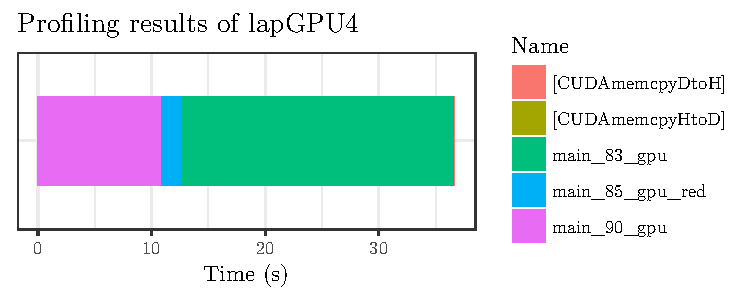
\includegraphics[width=0.7\textwidth]{images/timeline-gpu4}
	\caption{Timeline of the execution time of the GPU4 version, for \num{10000} iterations}
	\label{fig:timeline-gpu4}
\end{figure}

As a summary of these last versions, we can say that versions 2 and 3 are essentially the same, because the compiler already manages to optimise the order of the loops. and Version 4 does not add much to the performance, because of the limitation of the DRAM bandwidth.

%---------------------------------
\subsubsection{Optimisation: double buffer (\texttt{lapGPU5})}
For this version, is to use a double buffer. This allows us to avoid copying from \inline{Anew} to \inline{A} by reversing roles of \inline{A} and \inline{Anew} on every iteration:
\begin{lstlisting}[firstnumber=81]
if(iter % 2 == 0){
	#pragma acc kernels
	for( j=1; j < n-1; j++){
		for( i=1; i < m-1; i++ ){
			Anew[j][i] = ( A[j][i+1]+A[j][i-1]+A[j-1][i]+A[j+1][i])*0.25f;
			error = fmaxf( error, fabsf( Anew[j][i]-A[j][i] ) );}}
} else{
	#pragma acc kernels
	for( j=1; j < n-1; j++){
		for( i=1; i < m-1; i++ ){
			A[j][i] = ( Anew[j][i+1]+Anew[j][i-1]+Anew[j-1][i]+Anew[j+1][i])*0.25f;
			error = fmaxf( error, fabsf( A[j][i]-Anew[j][i] ) );}}
}
\end{lstlisting}

Then we compile with the PGI compiler as usual, and extract performance and metrics information:
\begin{lstlisting}[language=bash]
pgcc -fast -acc -ta=tesla:cc30 -Minfo=accel lapGPU5-double.c -o lapGPU5 &> lapGPU5-comp.log
nvprof ./lapGPU5 10000 2> lapGPU5-nvp.log
nvprof --kernels "main_84_gpu" --metrics sm_activity,inst_executed,l2_utilization, dram_utilization,dram_read_throughput,dram_write_throughput,ipc ./lapGPU5 100 2> lapGPU5-metrics.log
\end{lstlisting}

This is the next major improvement next to the loop fusion. In figure~\ref{fig:timeline-gpu5} we can clearly see how the execution is divided into two processes of computation and reduction. This is a clear indication that the double buffer works as intended.
\begin{figure}[H]
	\centering
	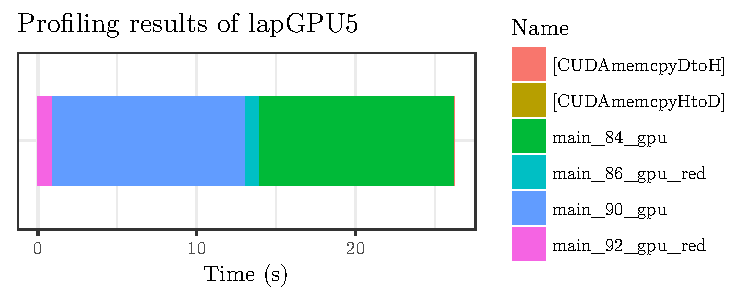
\includegraphics[width=0.7\textwidth]{images/timeline-gpu5}
	\caption{Timeline of the execution time of the GPU5 version, for \num{10000} iterations}
	\label{fig:timeline-gpu5}
\end{figure}

%---------------------------------
\subsubsection{Optimisation: parallel loop (vector 128) (\texttt{lapGPU6})}
Looking at \inline{lapGPU5-comp.log} we see we can still make a small optimisation to reduce the execution time: adding \inline{vector_length(128)} to the \inline{#pragma acc kernels} directives in lines 82 and 88 to force the size of the parallel loop:
\begin{lstlisting}[firstnumber=82]
#pragma acc kernels vector_length(128)
\end{lstlisting}

With this we make sure to divide the GPU into threads of the appropriate size to fully take advantage of our hardware.

Then we compile with the PGI compiler as usual, and extract performance and metrics information:
\begin{lstlisting}[language=bash]
pgcc -fast -acc -ta=tesla:cc30 -Minfo=accel lapGPU6-vec128.c -o lapGPU6 &> lapGPU6-comp.log
nvprof ./lapGPU6 10000 &> lapGPU6-nvp.log
nvprof --kernels "main_84_gpu" --metrics sm_activity,inst_executed,l2_utilization, dram_utilization,dram_read_throughput,dram_write_throughput,ipc ./lapGPU6 100 2> lapGPU6-metrics.log
\end{lstlisting}

In figure~\ref{fig:timeline-gpu6} we can see how the functioning to figure~\ref{fig:timeline-gpu5} is essentially the same. We just get a small time improvement.
\begin{figure}[H]
	\centering
	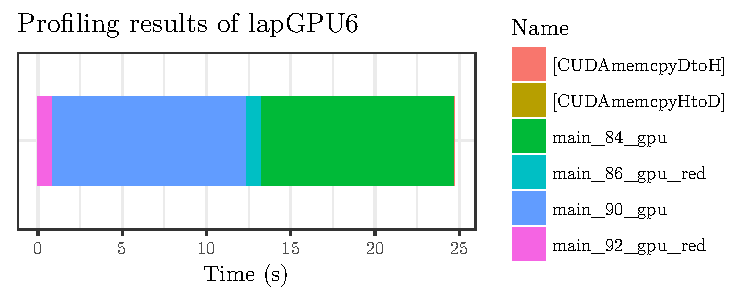
\includegraphics[width=0.7\textwidth]{images/timeline-gpu6}
	\caption{Timeline of the execution time of the GPU6 version, for \num{10000} iterations}
	\label{fig:timeline-gpu6}
\end{figure}

%---------------------------------
\subsubsection{Comparison of the GPU versions}
\begin{figure}[H]
	\centering
	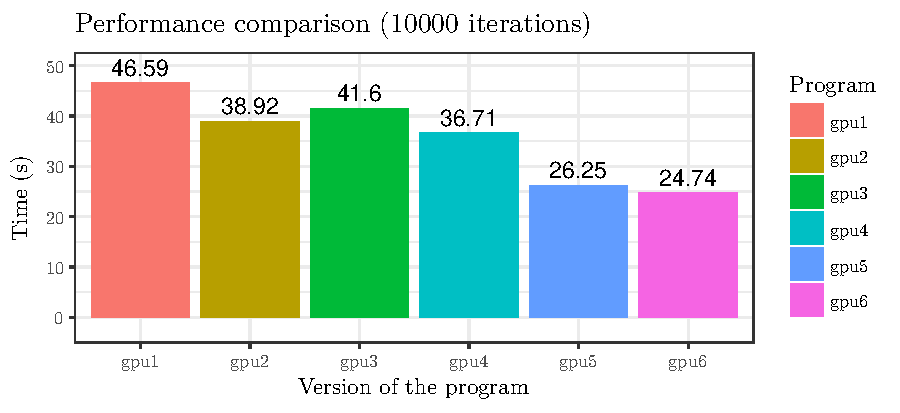
\includegraphics[width=0.9\textwidth]{images/times-gpu}
	\caption{Execution times of the GPU versions of the program}
	\label{fig:times-gpu}
\end{figure}

If we take a look at figure~\ref{fig:times-gpu}, we can compare the different implementations of GPU-oriented parallelisation and address its different results. It is relevant to note that not all implementations have been equally useful; as a matter of fact, some of them have been even counter-productive. Therefore, we  must consider the characteristics of the best implementations individually and highlight its importance.

The great improvements in the performance when using these different implementations are observed  in \inline{lapGPU2} and \inline{lapGPU5}. The former fuses different loops into a single loops, considerably reducing the operations needed to perform the same results; whilst the latter uses a double buffer in order to avoid carrying big matrices more times that needed, releasing a great deal of memory and hence easing the overall computation.

%---------------------------------
\subsubsection{Summary of the metrics}

In table~\ref{tab:metrics} below we can see a few conclusions can be extracted:
\begin{itemize}
	\item The biggest change is when implementing the loop fusion (\inline{GPU2}). The executed instructions are almost doubled, whilst the DRAM read/write throughput is halved. The IPC rate is a bit worse, but that does not have an important impact on the performance.
	\item For some reason, the loop inversion (\inline{GPU3}) has a pretty important, and bad, result on the performance as well as the metrics. The executed instructions were increased when compared to \inline{GPU2}, being this probably the reason of the increase in the execution time.
	\item Moving the square root out of the loop (\inline{GPU5}) improves a bit the DRAM read/write throughput and reduces the amount of executed instructions, as expected.
	\item Using the double buffer (\inline{GPU5}), even though makes a great performance improvement, does not make a big change on the metrics.
	\item Forcing the size of the parallel loop (\texttt{GPU6}) to 128 not only reduces the execution time, but the total executed instructions whilst improving the IPC rate.
\end{itemize}

\begin{table}[H]
	\centering
	\resizebox{\textwidth}{!}{
	\begin{tabular}{l c c c c c c}
	\toprule
	\toprule
	Version of the Program     & \texttt{GPU1}  & \texttt{GPU2}  & \texttt{GPU3}  & \texttt{GPU4}  & \texttt{GPU5}  & \texttt{GPU6}  \\
	\midrule
	Instructions Executed      & \num{24105472} & \num{46363722} & \num{50047882} & \num{43117312} & \num{43117312} & \num{41005504} \\
	L2 Cache Utilization       & Mid (6)        & Mid (4)        & Mid (4)        & Mid (4)        & Mid (4)        & Mid (4)        \\
	DRAM Utilization           & Mid (6)        & Low (3)        & Low (3)        & Low (3)        & Low (3)        & Mid (4)        \\
	DRAM Read (\si{GB\per\s})  & \num{50.161}   & \num{23.281}   & \num{23.149}   & \num{24.653}   & \num{24.658}   & \num{26.781}   \\
	DRAM Write (\si{GB\per\s}) & \num{51.078}   & \num{24.181}   & \num{23.979}   & \num{26.454}   & \num{26.455}   & \num{27.929}   \\
	Executed IPC               & \num{2.253070} & \num{2.001180} & \num{1.983949} & \num{1.972142} & \num{1.972746} & \num{2.037747} \\
	Multiprocessor Activity    & 99.72\%        & 99.86\%        & 99.87\%        & 99.86\%        & 99.86\%        & 99.85\%        \\
	\bottomrule
	\bottomrule
	\end{tabular}}
	\caption{Summary of the average metrics obtained with \inline{nvprof} for the different implementations of the program for GPU}
	\label{tab:metrics}
\end{table}

%-----------------------------------------------------------------
\subsection{Comparison of CPU vs GPU versions}
Until now we have discussed the different implementations used within a CPU-oriented parallelisation and their compared performances; nextly, we have stutdied the different implementations employed within a GPU-oriented parallelisation. Now it would be interesting to contrast the performances acquired between all different CPU and GPU oriented parallelisation implementations.
\begin{figure}[H]
	\centering
	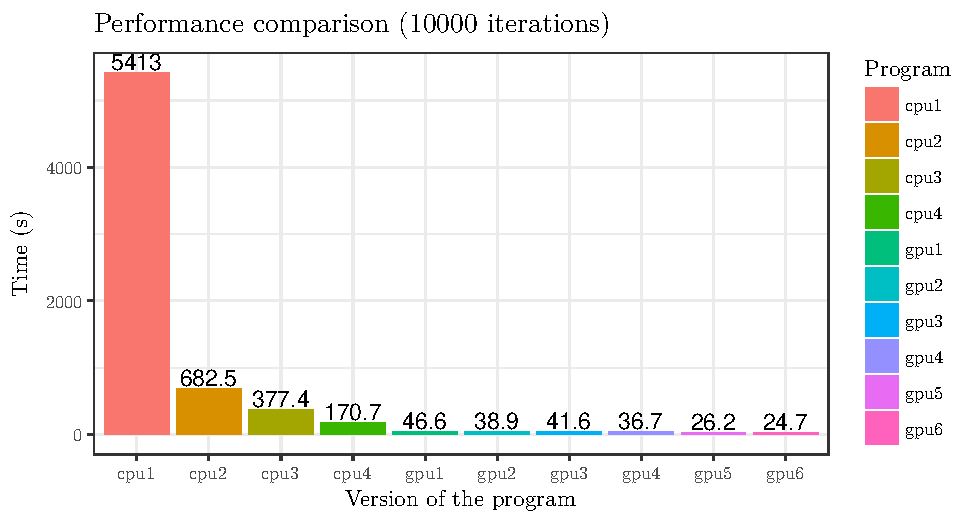
\includegraphics[width=0.95\textwidth]{images/times-all}
	\caption{Execution times of the CPU and GPU versions of the program}
	\label{fig:times-all}
\end{figure}

On figure~\ref{fig:times-all} above it is shown the execution times of all the different versions of the program. If we look closely at the figure, it is quite clear how dwarfed are the differences between the particular versions, when taking into account whether the version is CPU-oriented or GPU-oriented. The general conclusion extracted from this graph is that no matter how well implemented is a CPU parallelisation, the worst implementation using GPU is far better and it consumes considerably less computation time.

Despite that, some great improvements can be -- and should be -- acknowledged when well-implemented CPU parallelisation is used. This highlights the importance of a thorough parallelisation of the code, specially when no GPU is available.




%-----------------------------------------------------------------
%	CONCLUSIONS
%	!TEX root = ./../main.tex
%-----------------------------------------------------------------
\section{Conclusions}

During the resolution of this exercise, we have had the opportunity to manually create a parallel code, in contrast with the one we had optimised in the OpenMP assignment, that was itself an improvement from the very first code of the course. This time we have used a different methodology to paralellise the code, we have learned to take advantage of the GPU of our system, whose usage has increased dramatically over the past few years.

All of this has let us comprehend the importance of parallel programming when aiming for high performance computation, for we have experienced an incremental increase of the performance in the code we have been improving.

One of the most important things learn in this assignment has been the fact that one should not use OpenACC as a magic formula for improving the execution time of the code; one has to be aware of how the machine is working and optimise the code to really take advantage of the hardware capabilities of the system.


% \begin{appendices}
% \include{./contents/A-code}
% \end{appendices}

%-----------------------------------------------------------------
%	BIBLIOGRAPHY
%-----------------------------------------------------------------


\printbibliography[heading=bibintoc]
% \setcounter{secnumdepth}{0}
% \section{References}
% \printbibliography[title={Articles}, type=article, heading=subbibliography]
% \printbibliography[title={Books}, type=book, heading=subbibliography]
% \printbibliography[title={Websites}, type=online , heading=subbibliography]
% \printbibliography[title={Basic}, keyword=basic , heading=subbibliography]
% \printbibliography[title={Data Sets}, keyword=dataset , heading=subbibliography]
% \printbibliography[title={Licenses}, keyword=license , heading=subbibliography]

\end{document}
